%
% teil3.tex -- Beispiel-File für Teil 4
%
% (c) 2020 Prof Dr Andreas Müller, Hochschule Rapperswil
%
% !TEX root = ../../buch.tex
% !TEX encoding = UTF-8
%
\section{Bestimmung durch drei Punkte
\label{moebius:section:teil4}}
\kopfrechts{Bestimmung durch drei Punkte}


Eine Möbius-Transformation kann eindeutig durch die Abbildung von drei Punkten bestimmt werden.
Gegeben seien drei Punkte \( A, B, C \) in der komplexen Ebene sowie drei zugehörige Bildpunkte \( A', B', C' \). Dann existiert genau eine Möbius-Transformation, welche die Punkte \( A, B, C \) auf die Punkte \( A', B', C' \) abbildet.
Für zwei Punkte existieren unendlich viele Möbius-Transformationen, die diese Bedingung erfüllen. Für vier Punkte ist das Gleichungssystem im Allgemeinen überbestimmt und besitzt keine Lösung.
Eine Möbius-Transformation besitzt zwar vier Parameter \( a, b, c, d \), jedoch nur drei Freiheitsgrade, da eine gemeinsame Skalierung dieser Parameter die Transformation nicht verändert \cite{moebius:Moebiustransformationen}.
\index{Freiheitsgrad}%

\begin{proof}
Gegeben seien die Punkte
\[
A = z_1, \quad B = z_2, \quad C = z_3
\]
und die Bildpunkte
\[
A' = w_1, \quad B' = w_2, \quad C' = w_3.
\]
Die Möbius-Transformation hat die Form
\[
f(z) = \frac{az + b}{cz + d}.
\]
Wir bestimmen nun die Koeffizienten aus den Abbildungsbedingungen.
\\
1. Bedingung: \( A = z_1 \mapsto A' = w_1 \)
\[
w_1 = \frac{a z_1 + b}{c z_1 + d}
\quad \Rightarrow \quad
w_1(c z_1 + d) = a z_1 + b.
\]
2. Bedingung: \( B = z_2 \mapsto B' = w_2 \)
\[
w_2 = \frac{a z_2 + b}{c z_2 + d}
\quad \Rightarrow \quad
w_2(c z_2 + d) = a z_2 + b.
\]
3. Bedingung: \( C = z_3 \mapsto C' = w_3 \)
\[
w_3 = \frac{a z_3 + b}{c z_3 + d}
\quad \Rightarrow \quad
w_3(c z_3 + d) = a z_3 + b.
\]
Damit erhält man ein lineares Gleichungssystem in \(a,b,c,d\) (bis auf Skalierung).
Da eine Möbius-Transformation nur drei Freiheitsgrade besitzt, ist dieses System eindeutig lösbar (bis auf einen gemeinsamen Skalarfaktor).
Somit ist die Möbius-Transformation durch die drei Punktabbildungen eindeutig bestimmt.
\end{proof}

\begin{beispiel}
Gegeben seien die Punkte
\[
A = 0, \quad B = 1, \quad C = i
\]
und die Bildpunkte
\[
A' = 1 + i, \quad B' = 0, \quad C' = i.
\]
Die Möbius-Transformation hat die Form
\[
f(z) = \frac{az + b}{cz + d}.
\]
Wir bestimmen nun die Koeffizienten aus den Abbildungsbedingungen.
1. Bedingung:  \( A = 0 \mapsto A' = 1+i \)
\[
1+i = \frac{b}{d}
\quad \Rightarrow \quad
b = (1+i)d.
\]
2. Bedingung:  \( B = 1 \mapsto B' = 0 \)
\[
0 = \frac{a + b}{c + d}
\quad \Rightarrow \quad
a + b = 0
\quad \Rightarrow \quad
a = -b = -(1+i)d.
\]
3. Bedingung:  \( C = i \mapsto C' = i \)
\[
i = \frac{ai + b}{ci + d}.
\]
Durch Einsetzen von \( a \) und \( b \) erhalten wir
\[
i = \frac{-(1+i)di + (1+i)d}{ci + d}.
\]
Danach erfolgt das Faktorisieren von \( d \)
\[
i = \frac{d\left(-(1+i)i + (1+i)\right)}{ci + d}.
\]
Der Zähler vereinfacht sich zu
\[
-(1+i)i = -(i + i^2) = -(i - 1) = 1 - i
\]
\[
(1 - i) + (1 + i) = 2.
\]
Somit bekommt man
\[
i = \frac{2d}{ci + d}.
\]
Als nächstes folgt die Umformung
\[
i(ci + d) = 2d
\]
\[
ici + id = 2d
\]
mit \( i^2 = -1 \):
\[
ci^2 + id = 2d
\quad \Rightarrow \quad
-c + id = 2d.
\]
Nun lösen wir nach \(c\) auf:
\[
-c = 2d - id
\quad \Rightarrow \quad
c = (i - 2)d.
\]
Damit bleibt \(d \neq 0\) als Skalierungsfreiheit erhalten, und wir setzen ohne Beschränkung der Allgemeinheit \( d = 1 \).
Damit ergibt sich:
\[
a = -(1+i), \quad b = 1+i, \quad c = i-2, \quad d = 1.
\]
Damit ergibt sich die Möbius-Transformation
\[
f(z) = \frac{-(1+i)z + (1+i)}{(i-2)z + 1}.
\]
Alternativ faktorisiert erhält man
\[
f(z) = \frac{(1+i)(1 - z)}{1 + (i-2)z}.
\]
\emph{Überprüfung:}
Wir betrachten die konkrete Darstellung
\[
f(z)=\frac{(1+i)(1 - z)}{1 + (i-2)z}.
\]
Einsetzen der Punkte liefert
\begin{align*}
f(0) &= \frac{(1+i)}{1} = 1+i = A' \\
f(1) &= \frac{0}{1 + (i-2)} = 0 = B' \\
f(i) &= \frac{(1+i)(1-i)}{1 + (i-2)i}
\end{align*}
\[
(1+i)(1-i)=2
\]
\[
1 + (i-2)i = 1 + i^2 - 2i = 1 - 1 - 2i = -2i
\]
\[
f(i) = \frac{2}{-2i} = \frac{-1}{i} = i = C'.
\]
Damit wird gezeigt, dass die gewählte Möbius-Transformation die drei Punkte korrekt abbildet.
Die drei Freiheitsgrade einer Möbius-Transformation entsprechen genau den drei frei wählbaren Punktabbildungen. Dadurch ist eine Möbius-Transformation durch drei Punktpaare eindeutig bestimmt.
\end{beispiel}

\begin{figure}
	\centering
	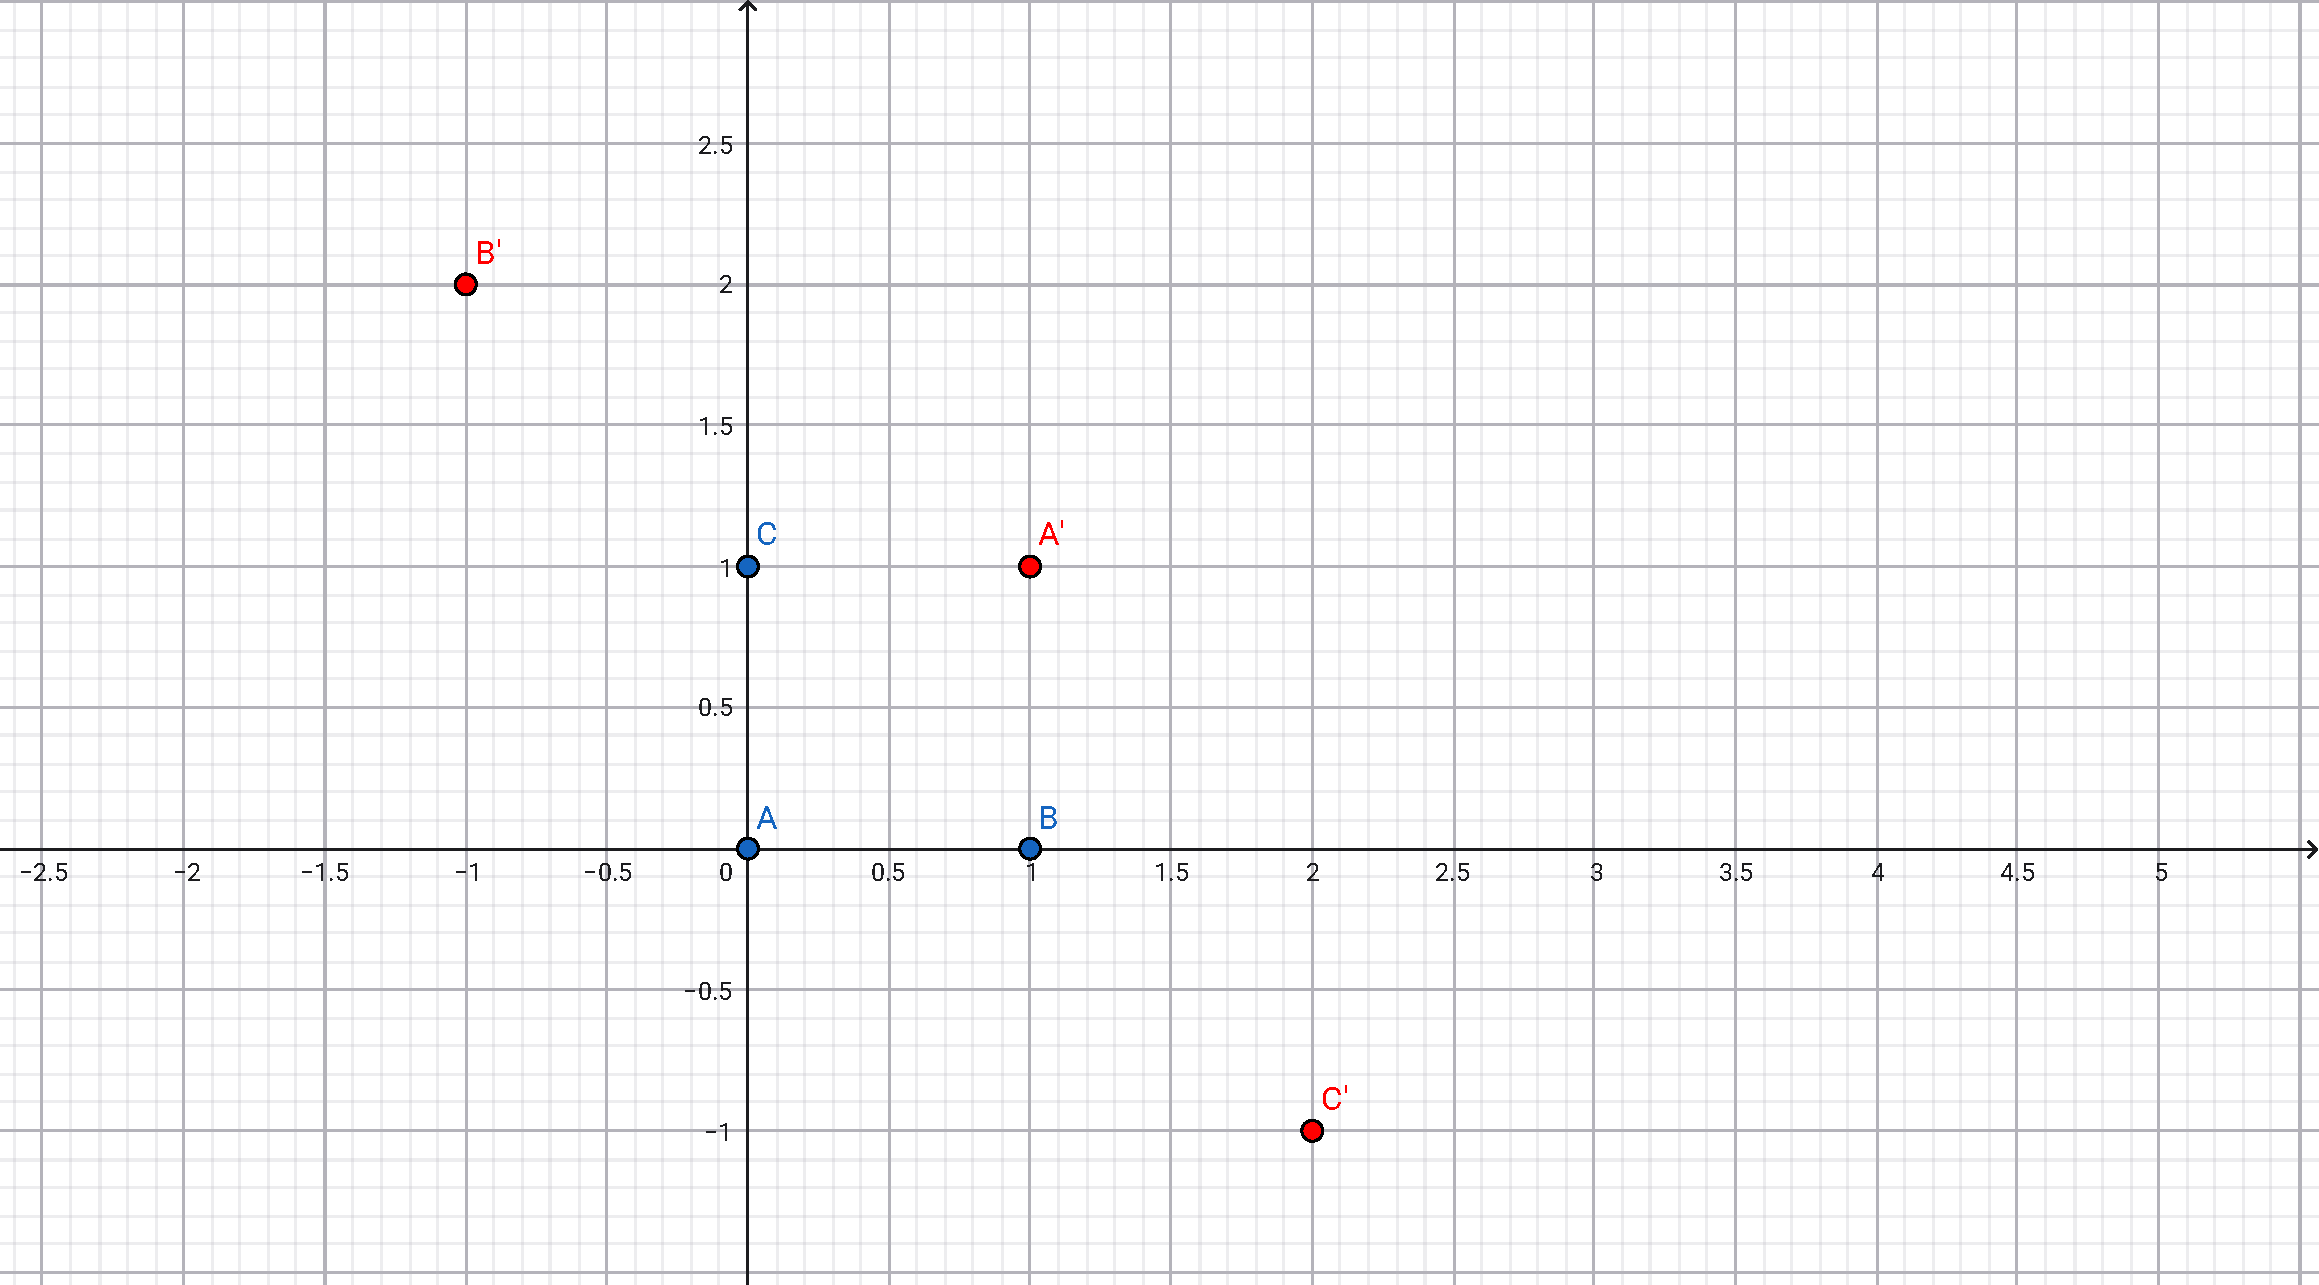
\includegraphics[width=1\textwidth]{papers/moebius/bild7.pdf}
	\caption{Graphische Darstellung vom Beispiel oben (erstellt mit GeoGebra)}
\end{figure}
